When we first deployed ORES, we reached out to several different wiki-communities and invited them to test out the system for use in patrolling for vandalism.  In these announcements, we encouraged editors to install ScoredRevisions,the only tool that used made use of ORES' edit quality models at the time.  ScoredRevisions both highlights edits that are likely to be damaging (as predicted by the model) and displays the likelihood of the prediction as a percentage.

Before long, our users began filing false-positive reports on wiki pages of their own design.  In this section we will describe three cases where our users independently developed these false-positive reporting pages and how they used them to understand ORES, the roles of automated quality control in their own spaces, and to communicate with us.

\subsection{Report mistakes (Wikidata)}
\begin{figure}[h]
  \centering
  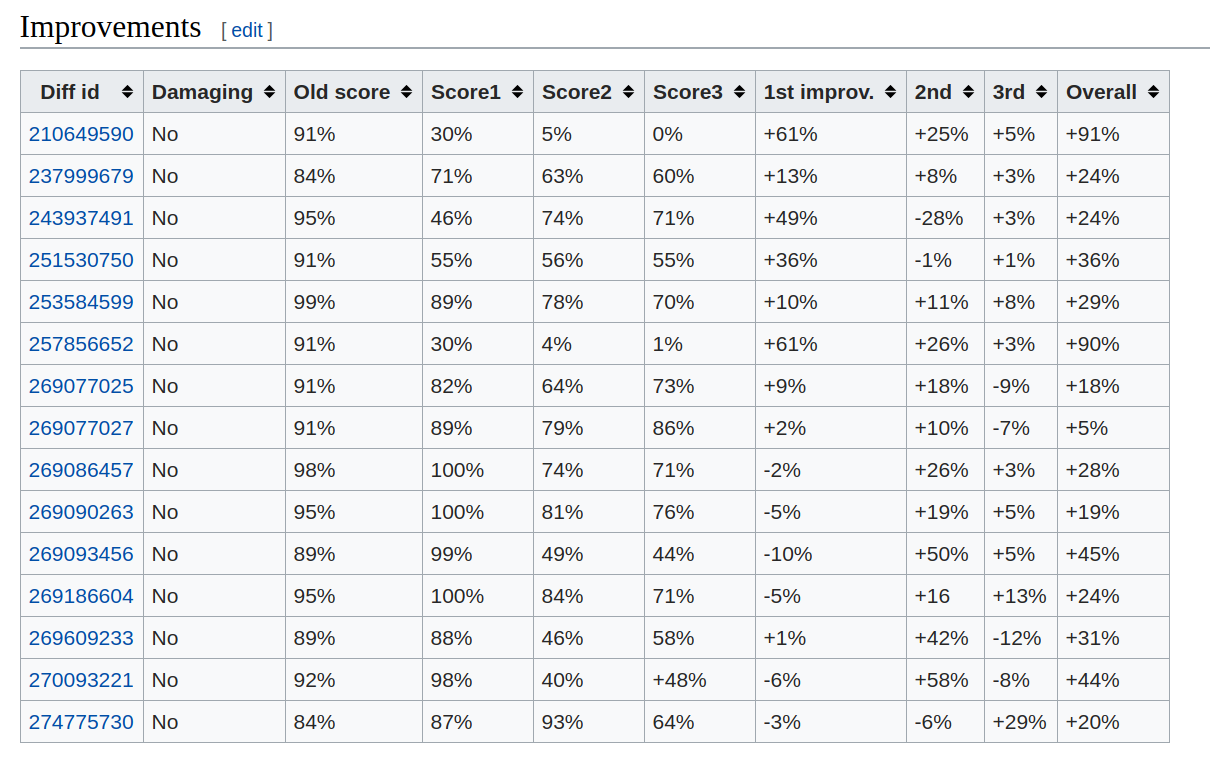
\includegraphics[width=.80\textwidth]{figures/ORES_report_mistakes_table}
  \caption{The ORES report mistakes table in Wikidata.}
  \label{fig:ores_report_mistakes}
\end{figure}

When we first deployed prediction models for Wikidata, a free and open knowledge base that can be read and edited by both humans and machines\footnote{\url{https://wikidata.org}}, we were breaking new ground by building a damage detection classifier based on a structured data wiki\cite{sarabadani2017building}.  So we created a page called ``Report mistakes'' and invited users to tell us about mistakes that the prediction model made on that page. We left the format and structure largely up to the users.

Within 20 minutes, we received our first report from User:Mbch that ORES was reporting edits that couldn't possibly be vandalism as potentially damaging.  As reports streamed in, we began to respond to them and make adjustments to the model building process to address data extraction bugs and to increase the signal so that the model differentiate damage from non-damaging edits.  After a month of reports and bug fixes, we decided to build a table to represent the progress that we made in iterations on the model against the reported false-positives.  See Figure~\ref{fig:ores_report_mistakes} for a screenshot of the table.  Each row represents a mis-classified edit, and each column describes the progress we made in not detecting those edits as damaging in future iterations of the model.  Through this process, we learned how Wikidata editors saw damage and how our modeling and feature extraction process captured signals in ways that differed from Wikidata editors' understandings.  We were also able to publicly demonstrate improvements to this community.

\subsection{Patrolling/ORES (Italian Wikipedia)}
Italian Wikipedia was one of the first wikis where we deployed basic edit quality models.  Our local collaborator who helped us develop the language specific features, User:Rotpunkt, created a page for ORES\footnote{\url{https://it.wikipedia.org/wiki/Progetto:Patrolling/ORES}} with a section for reporting false-positives (``falsi positivi'').  Within several hours, Rotpunkt and a few other edits started to notice some trends in their false positive reports.  First, Rotpunkt noticed that there were several counter-vandalism edits that ORES was flagging as potentially damaging, so he made a section for collecting that specific type of mistake (``annullamenti di vandalismo'').  A few reports later and he added a section for ''corrections to the verb for \emph{have}'' (``correzioni verbo avere'').  Through this process, editors from Italian Wikipedia were essential performing a grounded theory exploration of the general classes of errors that ORES was making.

Once there were several of these mistake-type sections and several reports within each section, Rotpunkt reached out to us to let us know what he had found.  He explained to us (via our IRC channel) that many of ORES mistakes were understandable, but there were some general trends in mistakes around the Italian verb for \emph{have}: ``ha''.  We knew immediately what was likely to be the issue.  It turns out that ``ha'' in English and many other languages is laughing, an example of informal language that doesn't belong in an encyclopedia article.  While the word ``ha'' in Italian translates to ``have'' and is perfectly acceptable in articles.

Because of the work of Rotpunkt and his collaborators in Italian Wikipedia, we were able to recognize the source of this issue (a set of features intended to detect the use of \emph{informal language} in articles) and to remove ``ha'' from that list for Italian Wikipedia.  This is just one example of many issues we were able to address because of the grounded theory and thematic analysis performed by Italian Wikipedians.

\subsection{PatruBOT (Spanish Wikipedia)}
Soon after we released support for Spanish Wikipedia, User:jem developed a robot to automatically revert damaging edits using ORES predictions (PatruBOT).  This robot was not running for long before our discussion pages started to be bombarded with confused Spanish-speaking editors asking us questions about why ORES did not like their work.  We struggled to understand the origin of the complaints until someone reached out to us to tell us about PatruBOT and its activities.

We haven't been able to find the source code for PatruBot, but from what we've been able to gather looking at its activity, it appears to us that PatruBOT was too sensitive and was likely reverting edits that ORES did not have enough confidence about.  Generally, when running an automated counter-vandalism bot, the most immediately operational concern is around \emph{precision} (the proportion of positive predictions that are true-positives).  This is because mistakes are extra expensive when there's no human judgement between a prediction and a revert (rejection of the contribution).  The proportion of all damaging edits that are actually caught by the bot (\emph{recall}) is a secondary concern to be optimized.

We recommend that bot developers who are interested in running an automated counter-vandalism bot use a threshold that maximizes recall at high precision (90\% is a good starting point).  According to our queries\footnote{\url{https://ores.wikimedia.org/v3/scores/eswiki?models=damaging&model_info=statistics.thresholds.true.\%27maximum\%20recall\%20@\%20precision\%20\%3E=\%200.9\%27}}, the Spanish Wikipedia damaging model can be expected to have 90\% precision and catch 17\% of damage if the bot only reverted edits where the likelihood estimate is above 0.959.

We reached out to the bot developer to try to help, but given the voluntary nature of their work, they were not available to discuss the issue with us.  Eventually, other editors who were concerned with PatruBOT's behavior organized an informal crowdsourced evaluation of the fitness of PatruBOT's behavior\footnote{\url{https://es.wikipedia.org/wiki/Wikipedia:Mantenimiento/Revisi\%C3\%B3n_de_errores_de_PatruBOT\%2FAn\%C3\%A1lisis}} where they randomly sampled 1000 reverts performed by PatruBOT and reviewed their appropriateness. At the time of writing, PatruBOT has been stopped\footnote{\url{https://es.wikipedia.org/wiki/Wikipedia:Caf\%C3\%A9\%2FArchivo\%2FMiscel\%C3\%A1nea\%2FActual\#Parada_de_PatruBOT}} and the informal evaluation is ongoing.

\subsection{Bias against anonymous editors}
Shortly after we deployed ORES, we started receiving reports that ORES' damage detection models were overly biased against anonymous editors.  At the time, we were using Linear SVM\footnote{\url{http://scikit-learn.org/stable/modules/generated/sklearn.svm.LinearSVC.html}} estimators to build classifiers, and we were considering making the transition towards ensemble strategies like GradientBoosting and RandomForest estimators\footnote{\url{http://scikit-learn.org/stable/modules/ensemble.html}}.  We took the opportunity to look for bias in the error of estimation between anonymous editors, newly registered editors.  By using our feature injection/interrogation strategy(described in Section~\ref{sec:innovations_in_openness}), we could ask our current prediction models how they would change their predictions if the exact same edit were made by a different editor.

\begin{figure}[h]
\centering
\begin{subfigure}[t]{.33\textwidth}
  \centering
  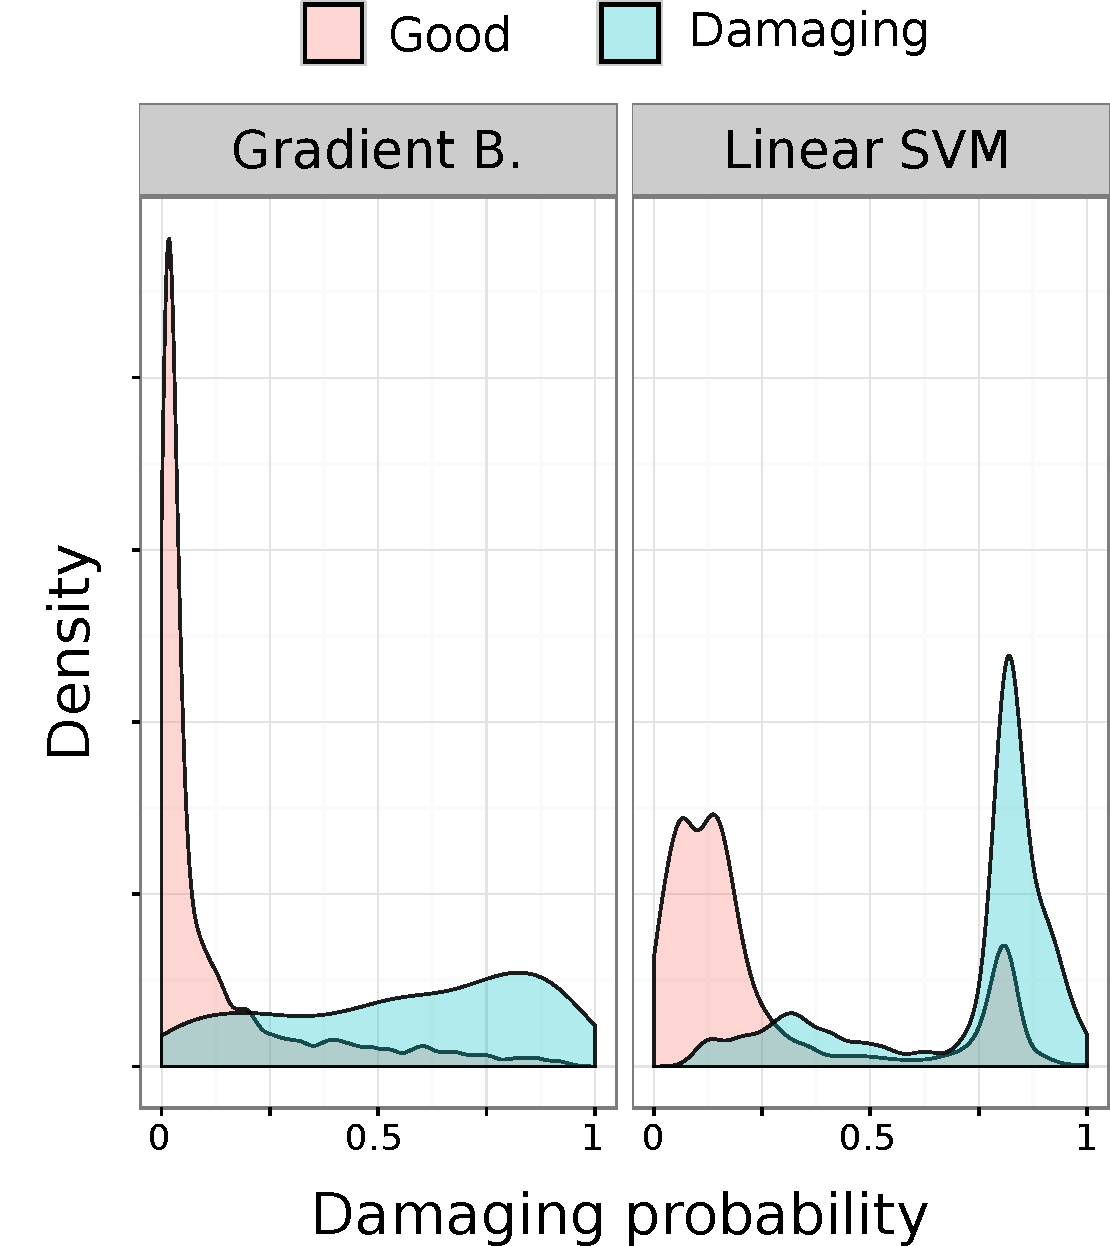
\includegraphics[width=.95\textwidth]{figures/natural_damaging_gb_vs_svc}
  \caption{No injected features}
  \label{fig:natural_damaging_gb_bs_svc}
\end{subfigure}~~
\begin{subfigure}[t]{.33\textwidth}
  \centering
  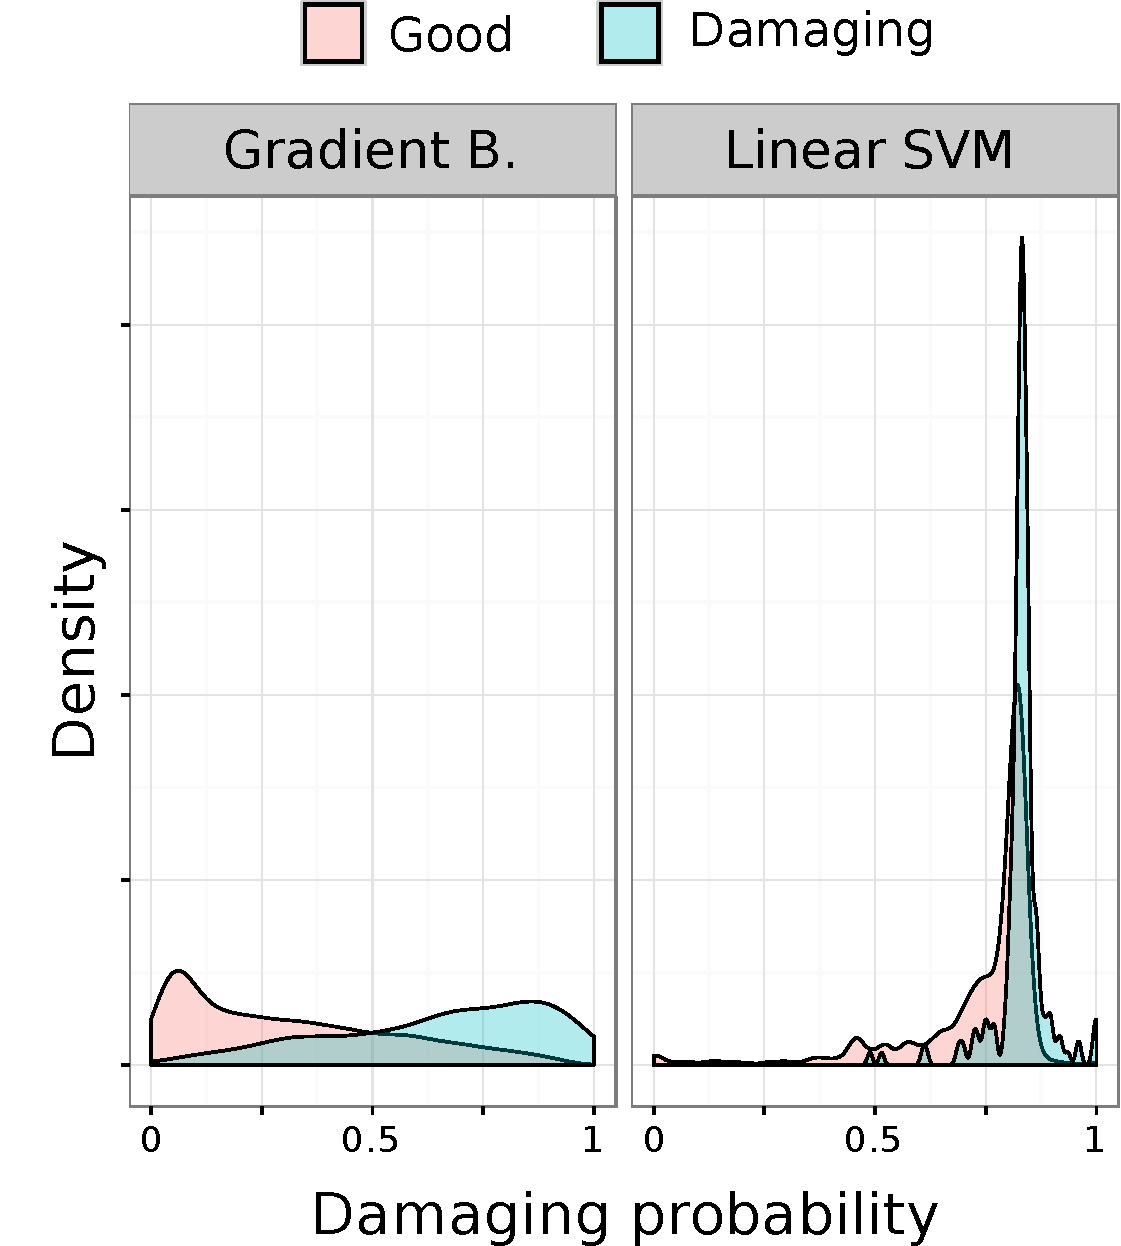
\includegraphics[width=.95\textwidth]{figures/anon_damaging_gb_vs_svc}
  \caption{Everyone is anonymous}
  \label{fig:anon_damaging_gb_bs_svc}
\end{subfigure}~~
\begin{subfigure}[t]{.33\textwidth}
  \centering
  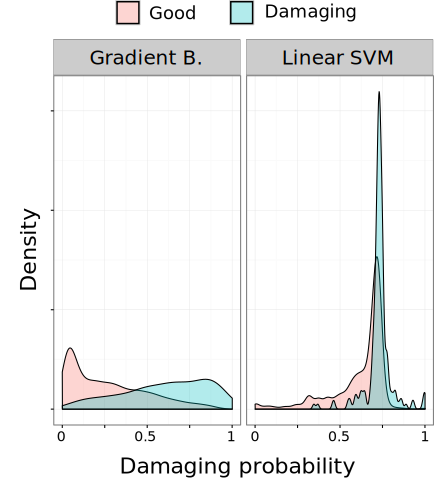
\includegraphics[width=.95\textwidth]{figures/newcomer_damaging_gb_vs_svc}
  \caption{Everyone is newly registered}
  \label{fig:newcomer_damaging_gb_bs_svc}
\end{subfigure}
\caption{The distributions of the probability of a single edit being scored as ``damaging'' based on injected features for the target user-class is presented.  Note that when injecting user-class features (anon, newcomer), all other features are held constant.}
\label{fig:prediction_error_for_anons_and_newcomers}
\end{figure}


Figure~\ref{fig:prediction_error_for_anons_and_newcomers} shows the probability density of the likelihood of ``damaging'' given three different passes over the exact same test set using two of our modeling strategies.  Figure~\ref{fig:natural_damaging_gb_bs_svc} shows that, when we leave the features to their natural values, it appears that both models are able to differentiate effectively between damaging edits (high damaging probability) and non-damaging edits (low damaging probability) with the odd exception of a large amount of non-damaging edits with a relatively high damaging probability around 0.8 in the case of the Linear SVM model.  Figures~\ref{fig:anon_damaging_gb_bs_svc} and \ref{fig:newcomer_damaging_gb_bs_svc} show a stark difference.  For the scores that go into these plots, characteristics of anonymous editors and newly registered editors were injected for all of the test edits.  We can see that the GradientBoosting model can still differentiate damage from non-damage while the Linear SVM model flags nearly all edits as damage in both case.

Through the reporting of this issue and our subsequent analysis, we were able to identify the issue and show that an improvement to our modeling strategy mitigates the problem.  Without such a tight feedback loop, we most likely wouldn't have noticed how poorly ORES' damage detection models were performing in practice.  Worse, it might have caused vandal-fighters to be increasingly (and inappropriately) skeptical of contributions by anonymous editors and newly registered editors---two groups of contributors that are already met with unnecessary hostility\footnote{\url{http://enwp.org/:en:Wikipedia:IPs_are_human_too}}\cite{halfaker2013rise}.

\subsection{Discussion}
These case studies in responses to ORES provide a window into how our team has been able to work with the locals in various communities to refine our understandings of their needs, into methods for recognizing and addressing biases in ORES' models, and into how people think about what types of automation they find acceptable in their \emph{spaces}.

\leadin{Refining our understandings and iterating our models}
The information divide between us researchers/engineers and those members of a community is often wider than we realize.  Through iteration with the Wikidata and Italian models, we learned about incorrect assumptions we would made about how edits happen (e.g. client edits in Wikidata) and how language works (e.g. ``ha'' is not laughing in Italian).  It's likely we would never be able to fully understand the context in which damage detection models should operate before deploying the models.  But these case studies demonstrate how, with a tight communication loop, many surprising and wrong assumptions that were baked into our modeling process could be identified and addressed quickly.  It seems that many of the relevant issues in feature engineering and model tuning become apparent when the model is used in context to try to address a real problem (in these cases, counter-vandalism).

\leadin{Methods for recognizing and addressing bias}
The Italian Wikipedians showed us something surprising and interesting about collaborative evaluation of machine prediction: thematic analysis is very powerful.  Through the collection of ORES mistakes and iteration, our Italian collaborators helped us understand general trends in the types of mistakes that ORES made.  It strikes us that this a somewhat general strategy for bias detection.  While our users certainly brought their own biases to their audit of ORES, they were quick to discover and come to consensus about trends in ORES' issues.  Before they had performed this process and shared their results with us, we had no idea that any issues was present.  After all, the fitness statistics for the damage detection model looked pretty good---probably good enough to publish a research paper!  Their use of thematic analysis seems to like a powerful tool that developers will want to make sure is well supported in any crowd based auditing support technologies.

\leadin{How people think about ``acceptable'' automation}
In our case study, Spanish Wikipedians are in the processes of coming to agreements about what roles are acceptable for automated agents.  Through observation of PatruBOT's behavior, they have decided that the \emph{false discovery rate} (i.e., $1 - \text{precision}$) was too high by watching the bot work in practice and they started their own independent analysis to find quantitative, objective answers about what the real rate is.  Eventually they may come to a conclusion about an acceptable \emph{false discovery rate} or they may decide that no revert is acceptable without human intervention.
